%==============================================================================
\section{Experiments}
\label{sec:exp}
%==============================================================================

All schemes share the model of Section~\ref{sec:model}: per-device peak power, real noise of unit variance per stream and $\snr=P$. ``Required SNR'' is the smallest SNR at which a metric reaches a target, interpolated linearly between grid points; ``--'' means that the target is not met on the grid. Unless stated otherwise, the ladder step is $\Delta=3$~dB, the tone handshake uses $\nu=4$ REs per level and $\alpha=10^{-3}$, and the digital handshake uses $q=256$ with its false zeros simulated. ``Proposed'' denotes Algorithm~\ref{alg:ladder} with both components and $\kappa=1$. Code and raw results are available at \url{https://github.com/zr0212-boom/aircomp-softmax}.

\subsection{Verification of the Analysis}

Every closed form was verified by Monte Carlo with $4\times10^5$--$10^6$ trials (69 checks), for uniform, geometric and attention-like weight profiles with and without heterogeneous path loss: the law~\eqref{eq:bottleneck} of $B$, its forms for $C=2,4$ coherence blocks and for the noise-matched report~\eqref{eq:kappa_law} with $\kappa\in\{0.3,1,3\}$, and the Nakagami law~\eqref{eq:bottleneck_m}, all within a CDF error of $2.2\times10^{-3}$; the distortion bound of Proposition~\ref{prop:kappa}(i), which is attained; the saturation law~\eqref{eq:psat} and its two other forms; both outage expressions of Theorem~\ref{thm:outage}; the bounds of Proposition~\ref{prop:combiner}; the false-alarm and miss probabilities of Proposition~\ref{prop:detection} within 4\% and 3\%; and Theorem~\ref{thm:converse}, where the ladder meets $W/(2K)$ on a uniform range and the optimum found by dynamic programming for Gaussian $X$ is within 4\% of the high-resolution value.

\subsection{Sharded-KV LLM Decoding}

\emph{Setup.} We use Qwen3-4B-Instruct and Qwen3-8B~\cite{qwen3} and Llama-3.1-8B-Instruct~\cite{llama3} in bfloat16; all have $H=32$ query heads with $d_v=128$. The FC holds the first 64 tokens and everything from the question on; the context in between is split into $N$ contiguous shards, and the attention of every query from the question on, in every layer and head, is merged over the air. In the fidelity task, the last 256 positions of a $T$-token text from WikiText-103~\cite{merity2017wikitext} are teacher-forced and compared with the exact shard merge, over 4 text segments and 4 channel draws, i.e., 16 samples per configuration. Channels are i.i.d.\ Rayleigh per layer and position and shared by the heads of a layer; $\sigma_o$, $V_{\max}$ and the ladder range are calibrated per layer and head on a disjoint text. The target is an NLL increase of 0.05~nats. The bfloat16 difference between the exact merge and the native attention kernel, a KL divergence of $5\times10^{-4}$--$10^{-3}$, bounds the resolution of any comparison. All schemes of a configuration see the same segments, channels and noise, so we report differences of required SNRs with paired bootstrap intervals (2000 resamples), which are tighter than those of the individual values (about $\pm1.5$~dB). The SNR grid is $-15$ to 25~dB in steps of 2.5~dB (from 0~dB for the designs that need more than that).

\emph{Baselines.} Three known-weight baselines reveal every $d_j$ to the FC: the genie scale~\eqref{eq:genie} with the exact denominator; the threshold scale of AirMoE~\cite{yang2026airmoe}, solved exactly per instance, with the exact denominator; and ``AirMoE-eff'', the same scale with the denominator of the arrived weights, i.e., AirMoE strengthened with our component~A. The private-weight references are the analog ladder and the non-saturating split ratio with its overflow fallback and consistency check, both with the tone handshake.

\emph{Choice of $\kappa$.} The rule was fixed before the test runs: on the CPython documentation as development corpus (Qwen3-4B, 8k, $N=8,32,64$), take the better of $\kappa=0.3$ and $\kappa=1$ by the mean required SNR on the 0--25~dB grid. The result was $\kappa=1$ (0.7 against 1.5~dB), which is used for every model, context length and $N$ on WikiText.

\begin{table*}[t]
\centering
\caption{SNR (dB) at which the NLL increase falls to 0.05~nats, $M=4$. Known-weight designs reveal every $d_j$ to the FC. Gaps: required SNR of the proposed design with the digital handshake minus that of the best known-weight design (AirMoE-eff; $^\dagger$AirMoE) and minus that of the non-saturating split ratio, with paired 95\% bootstrap intervals.}
\label{tab:llm}
\setlength{\tabcolsep}{3.5pt}
\begin{tabular}{@{}lcc ccc cccc cc@{}}
\toprule
 & & & \multicolumn{3}{c}{Known weights} & \multicolumn{4}{c}{Private weights} & \multicolumn{2}{c}{Gap of proposed (digital) to} \\
\cmidrule(lr){4-6}\cmidrule(lr){7-10}\cmidrule(l){11-12}
Model & Context & $N$ & Genie & AirMoE & AirMoE-eff & \shortstack{Analog\\ladder} & \shortstack{Non-sat.\\split} & \shortstack{Proposed\\(tone)} & \shortstack{Proposed\\(digital)} & best known weights & non-sat.\ split \\
\midrule
\tabinput{tables/tab_llm}
\bottomrule
\end{tabular}
\end{table*}

\emph{Fidelity.} Table~\ref{tab:llm} lists the required SNRs and Fig.~\ref{fig:llm} the curves of one configuration. Five observations hold for all models and context lengths. First, the proposed design with the digital handshake needs $-8.4$ to $8.4$~dB, which is 4.7--12.3~dB less than the non-saturating split ratio, with every interval excluding zero, and 9--16~dB less than the analog ladder. Second, it needs 1.8--9.1~dB less than known-weight aggregation at the genie scale and is on par with or better than AirMoE with the exact denominator ($-7.7$ to $+1.3$~dB): a private design that lets devices saturate in a controlled way outperforms a known-weight design that does not. Third, the strongest baseline, AirMoE-eff, remains 0.2--4.1~dB ahead (1.0--3.0~dB for Qwen3-4B, 0.2--2.6~dB for Llama-3.1-8B, 0.3--4.1~dB for Qwen3-8B); the interval includes zero in 3 of the 24 configurations. This is the price of private weights: a per-device budget cannot balance the total distortion against the noise as the centralized threshold does. Fourth, the tone handshake costs 0.7--11.7~dB relative to the digital one, most for Llama-3.1-8B, whose operating point is lowest: the proposed design then operates where tones are missed (for Qwen3-4B at 0~dB, the detected level is below the true one in 76--91\% of the instances), and although component~A keeps the misses harmless in the sense of Proposition~\ref{prop:eff}, the scale is no longer matched to the noise. The tone variant is still 0.2--5.1~dB better than the non-saturating split ratio with the same tones. Fifth, the required SNR does not grow with the number of devices: for Qwen3-4B at 8k it is 1.2, 2.8, 2.0, 1.5, 0.7 and $-0.1$~dB for $N=4$ to 128, whereas time-division ZF, which meets the target at about 0~dB, needs $\lceil2N/M\rceil$ slots. Longer contexts cost more: from 8k to 32k at $N=32$, the proposed design loses 5--8~dB and AirMoE-eff 4--10~dB. With $M=8$ antennas (Qwen3-4B, 8k), it needs 1.2, $-0.1$ and $-0.1$~dB for $N=8$, 32 and 64, i.e., 0.8--1.6~dB less than with four, at gaps of 1.0--2.8~dB to AirMoE-eff.

The attention statistics explain the size of these gains. With unit gains, $\log_{10}S$ spans 2.0--2.3 decades between the 10th and 90th percentiles of the decode positions in the median head and 3.1--3.7 decades in the 90th-percentile head, and the participation ratio is small (median $\Neff$ of 2.0--3.1, 4.5--8.3 and 6.4--13.8 for $N=8$, 32 and 64 at 8k): a few shards hold the mass, and the bottleneck is typically set by a device whose contribution to the output is minor. At the operating point of the proposed design nearly every instance has a saturated device (96--100\% at 0--5~dB for Qwen3-4B), yet the saturated mass $\sum_j(d_j-a_j)$ is only 5--10\% of the denominator.

\begin{figure}[t]
\centering
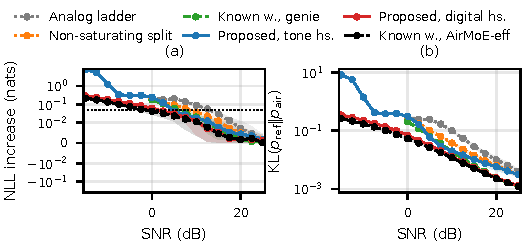
\includegraphics[width=\linewidth]{fig_llm_curves.pdf}
\caption{Qwen3-4B, 8k context, $N=32$ devices, $M=4$: (a) NLL increase and (b) KL divergence versus SNR (4 segments $\times$ 4 channel draws; shaded: 95\% confidence interval).}
\label{fig:llm}
\end{figure}

\emph{Design study.} Table~\ref{tab:design} separates the components for Qwen3-4B at 8k. Component~A alone changes little ($-1.0$ to $0.0$~dB against the non-saturating split ratio), as expected: it makes saturation harmless but does not create any. Component~B creates it: with both components the required SNR falls by 3.9--7.0~dB with the digital handshake and by 1.4--3.8~dB with tones. With the digital handshake, B with the exact denominator is as good as A+B (differences of $-0.1$ to $+0.3$~dB, intervals within $\pm1.3$~dB), in line with Proposition~\ref{prop:kappa}(i); with tones, B needs A: the analog denominator is 1.3--3.7~dB worse. The noise-matched rule is also as good as or better than a fixed 3~dB offset of the scale (by 0.1--1.1~dB). In $\kappa$ the design is monotone over the tested range: $\kappa=3$ is a further 0.6--1.1~dB better than the pre-registered $\kappa=1$ on this configuration, so the reported numbers are not tuned to the test set and leave some margin. A step of 6~dB costs 0.8--1.2~dB and a step of 1.5~dB gains 0.4~dB, consistent with the mean quantization penalty $\Delta/2$ of Theorem~\ref{thm:converse}, so the ladder can be halved at about 1~dB. For the tones, $\nu=8$ instead of 4 gains 1.1--1.3~dB and $\nu=2$ loses 1.4--1.9~dB. Component~A is worth 1.0--3.1~dB to the AirMoE baseline as well.

\begin{table}[t]
\centering
\caption{Design study, Qwen3-4B, 8k, $M=4$: required SNR (dB). A: saturation-aware denominator; B: noise-matched report.}
\label{tab:design}
\setlength{\tabcolsep}{2.5pt}
\begin{tabular}{@{}lccc@{}}
\toprule
Design & $N=8$ & $N=32$ & $N=64$ \\
\midrule
\tabinput{tables/tab_design}
\bottomrule
\end{tabular}
\end{table}

\emph{One-round designs.} Can the handshake round be saved? Not with the designs we know. The best blind scale, a fixed quantile of $B$ chosen on the test set, needs 27.5--28.4~dB for Qwen3-4B (19.3--19.5~dB for Llama-3.1-8B, 28.2--28.5~dB for Qwen3-8B); the 0.5 quantile never reaches the target and the 0.99 quantile fails or needs 31--47~dB, which is the dilemma of Corollary~\ref{cor:blind}. Component~A lowers the best blind scale to 22.5--23.3~dB, and a stale ladder that reuses the level of the previous position needs 23.2--28.3~dB with A, with or without B. The handshake is thus worth more than 20~dB.

\emph{Channel impairments.} Table~\ref{tab:real} repeats the $N=32$ configuration under impairments; phase and CSI errors use the I/Q model of Section~\ref{sec:regime}, including the leakage between quadrature streams. Independent channels per head and channels that stay constant over the session cost nothing. Spanning $C=2$ and 4 coherence blocks costs the proposed design 2.2 and 4.7~dB and the known-weight designs 2.0--2.8 and 3.8--5.4~dB, against the 3 and 6~dB of Corollary~\ref{cor:coherence} for a non-saturating scale. Phase errors of up to $10^\circ$, ramps of up to $45^\circ$ across the payload and a CSI error of 0.05 cost the proposed design at most 0.6~dB; $20^\circ$ and an NMSE of 0.1 cost 1.5 and 2.4~dB, whereas the non-saturating split ratio loses 4.2 and 9.6~dB. A large-scale spread of 4 and 8~dB costs 2.2 and 9.3~dB, of which the digital fallback of the two weakest devices recovers 2.5 and 2.7~dB; the known-weight baselines lose as much (2.7 and 9.6~dB for AirMoE-eff), so the spread is a property of the task rather than of private weights. With all impairments combined, the proposed design needs 4.2~dB for Qwen3-4B and $-0.9$~dB for Llama-3.1-8B. Across all rows the gap to AirMoE-eff stays between 1.4 and 3.0~dB.

\begin{table}[t]
\centering
\caption{Channel impairments, Qwen3-4B, 8k, $N=32$, $M=4$: required SNR (dB). Spread: log-normal large-scale gains. Combined: per-head channels, $C=2$, phase error $10^\circ$, ramp $20^\circ$, CSI NMSE 0.01 and 4~dB spread; fallback: 4 / 8~dB spread.}
\label{tab:real}
\setlength{\tabcolsep}{2.5pt}
\begin{tabular}{@{}lccccc@{}}
\toprule
 & \multicolumn{2}{c}{Known weights} & \multicolumn{3}{c}{Private weights} \\
\cmidrule(lr){2-3}\cmidrule(l){4-6}
Scenario & Genie & \shortstack{AirMoE\\-eff} & \shortstack{Non-sat.\\split} & \shortstack{Prop.\\(tone)} & \shortstack{Prop.\\(dig.)} \\
\midrule
\tabinput{tables/tab_real}
\bottomrule
\end{tabular}
\end{table}

\emph{Retrieval.} In the needle-in-a-haystack task, one or four passphrases are placed at depths of 10\%, 50\% and 90\% of a WikiText haystack, with 60 prompts and 2 channel draws (120 trials). A trial succeeds if every token of the exact-merge answer is the arg-max under the over-the-air merge, which is equivalent to greedy decoding with the same channel draws (against greedy generation the difference is $+0.5\pm0.4$ percentage points over 8 configurations). Table~\ref{tab:niah} reports the accuracy. With the digital handshake the proposed design is within one trial of the ceiling from 10~dB on in all 16 configurations (Table~\ref{tab:niah} lists those with $N\ge32$) and loses at most 1.7 points with one key and 3.3 points with four keys at 5~dB; in no cell is it below AirMoE-eff. With tones it needs 10~dB to come within two trials of the ceiling and fails at 5~dB with four keys.

\begin{table}[t]
\centering
\caption{NIAH accuracy (\%), teacher-forced, 120 trials, $M=4$. Ceiling: teacher-forced accuracy without the channel.}
\label{tab:niah}
\setlength{\tabcolsep}{1.7pt}
\begin{tabular}{@{}lcccccccc@{}}
\toprule
 & & \multicolumn{2}{c}{AirMoE-eff} & \multicolumn{2}{c}{Prop.\ (dig.)} & \multicolumn{3}{c}{Prop.\ (tone)} \\
\cmidrule(lr){3-4}\cmidrule(lr){5-6}\cmidrule(l){7-9}
Model, context, $N$ & Ceil. & 5 & 10 & 5 & 10 & 5 & 10 & 15~dB \\
\midrule
\tabinput{tables/tab_niah}
\bottomrule
\end{tabular}
\end{table}

\subsection{Secure Digital Merge and Latency}

\emph{Ring size at matched accuracy.} We implemented the secure digital merge in fixed point, on an error-free link, and searched the ring size $b$ at which the NLL increase stays below 0.05~nats for every $N$. With an offline scale per head (the calibrated maximum with an 8-bit margin for queries outside the calibration range), it needs 32~bits for Qwen3-4B at 8k, 36~bits at 32k and 28~bits for the two 8B models. With an oracle scale per instance, a lower bound for any public scale, 10--12~bits suffice. A plain bfloat16 merge also meets the target.

\emph{Latency.} Table~\ref{tab:latency} evaluates Section~\ref{sec:regime} for Qwen3-4B (36 layers) at an operating SNR of 15~dB with the required SNRs of the 8k sweep, $\tau=0.5$~ms, an RE efficiency of 0.72, a digital rate of Shannon capacity minus 3~dB with $\min(M,N)$-fold multiplexing, which favors the digital schemes, $L=32$, $b_A=\FXBITS$ and $b_w=16$~bits. The secure digital merge is given its measured ring sizes; for the per-instance scale we charge the second round trip but not the handshake payload. At 20~MHz the proposed design, in the faster of its two forms, is 1.4--14.5 times faster than the per-instance secure merge for $N=4$ to 128 and 2.4--42 times faster than the offline-scale one; at 100~MHz the factors are 1.1--5.4 and 0.95--14, the only exception being $N=4$, where the offline-scale merge is 5\% faster. The digital handshake is the faster form up to $N=8$; beyond that its $NHL$ bytes dominate and the tone handshake, whose cost does not depend on $N$, is preferable. Schemes that reveal the weights or the per-device data remain faster: known-weight aggregation by 1--18~ms, and time-division ZF for $N\le8$ at 20~MHz and $N\le32$ at 100~MHz (Fig.~\ref{fig:regime}).

\begin{table}[t]
\centering
\caption{Per-token latency (ms) at matched accuracy, Qwen3-4B, $M=4$, SNR 15~dB. Private schemes reveal neither weights nor per-device data. Secure digital merge: 12-bit ring with a per-instance scale (lower bound) and 36-bit ring with an offline scale.}
\label{tab:latency}
\setlength{\tabcolsep}{2.5pt}
\begin{tabular}{@{}lccccccc@{}}
\toprule
 & \multicolumn{4}{c}{Private} & \multicolumn{3}{c}{Not private} \\
\cmidrule(lr){2-5}\cmidrule(l){6-8}
 & \multicolumn{2}{c}{Proposed} & \multicolumn{2}{c}{Secure dig.} & Known & ZF- & Dig. \\
Band, $N$ & dig. & tone & inst. & offl. & w. & TDMA & bf16 \\
\midrule
\tabinput{tables/tab_latency}
\bottomrule
\end{tabular}
\end{table}

\subsection{Spatial-Field Estimation}

\emph{Setup.} As in~\cite{sato2026awa}, a log-normal shadowing field (8~dB, Gudmundson correlation distance 100~m~\cite{gudmundson1991correlation}) covers $500\times500$~m$^2$ and measurements carry 1~dB noise; each round estimates the field at 10 query points that share one channel draw, and we report the median per-round RMSE over 2000 rounds. In product-of-experts (PoE) regression, 256 measurements are partitioned among $K$ devices by a grid, with the local posterior precisions as weights; in Nadaraya--Watson (NW) regression, each of $K$ sensors holds one measurement (bandwidth 30~m) and the FC adds a prior pseudo-observation. Adaptively weighted averaging (AWA)~\cite{sato2026awa} clips the weights to bounds tuned per SNR on a calibration set, an optimistic stand-in for its Bayesian optimization. ``Ladder-T'' is the analog ladder with weak-link truncation~\cite{zhu2020broadband}: devices whose gain is below a tuned quantile are not scheduled. The proposed design uses the same $\kappa=1$ and $\Delta=3$~dB as for the LLMs, without any tuning, and 16 tone observations per level.

\emph{Results.} Table~\ref{tab:field} summarizes the single-antenna results. With equal path loss the proposed design is within 0.13~dB of AirMoE-eff at 10~dB with either handshake and outperforms AWA by 0.4--1.6~dB. With a 10~dB log-normal spread of the large-scale gains (unit mean), non-saturating designs collapse, since a few devices with weak links dominate $S=\sum_jd_j^2/\beta_j$: the genie scale with known weights is at 8.7--15.9~dB at 10~dB. The noise-matched report caps these devices by itself: the proposed design stays within 0.02--1.7~dB of AirMoE-eff (digital handshake; at most 0.7~dB with tones) and outperforms AWA by 3.5--16~dB at 10~dB. Without any tuning it is within 0.1~dB of the tuned truncation or better in all entries but one (PoE with $K=4$ at 10~dB). With few devices and a large spread, tones do better than the digital handshake at 10--20~dB because the tones of the weakest devices go undetected, an implicit truncation; at 0~dB the same effect makes the tone variant fail for PoE with $K=4$.

\begin{table*}[t]
\centering
\caption{Spatial-field estimation: median RMSE (dB) at 10 / 20~dB, $M=1$. Spread: unit-mean log-normal large-scale gains with 10~dB standard deviation. AirMoE-eff knows every weight; Ladder-T and AWA are tuned per SNR.}
\label{tab:field}
\setlength{\tabcolsep}{5pt}
\begin{tabular}{@{}llccccccc@{}}
\toprule
Path loss & Task, $K$ & Ideal & AirMoE-eff & Proposed (digital) & Proposed (tone) & Non-sat.\ split & Ladder-T & AWA~\cite{sato2026awa} \\
\midrule
\tabinput{tables/tab_field}
\bottomrule
\end{tabular}
\end{table*}
